\documentclass[11pt]{article}
\usepackage[T1]{fontenc}
\usepackage{lmodern,amsmath,amssymb,amsthm,booktabs,microtype}
\usepackage[margin=1in]{geometry}
\usepackage{tikz}
\usetikzlibrary{arrows.meta,patterns}
\usepackage[colorlinks=true,linkcolor=blue,citecolor=blue,urlcolor=blue]{hyperref}
\newtheorem{theorem}{Theorem}[section]
\newtheorem{lemma}[theorem]{Lemma}
\newtheorem{corollary}[theorem]{Corollary}
\newtheorem{proposition}[theorem]{Proposition}
\theoremstyle{remark}\newtheorem{remark}[theorem]{Remark}
\newcommand{\R}{\mathbb R}
\newcommand{\sgn}{\operatorname{sgn}}
\newcommand{\diag}{\operatorname{diag}}
\newcommand{\degB}{\operatorname{deg}}
\newcommand{\one}{\mathbf 1}
\title{A determinant dichotomy for quadratic zero-one systems:\\steady-state parity, boundedness, and finite-time escape}
\author{Vamshi Jandhyala\\\small London, United Kingdom}
\date{Preprint v1, 20 October 2026}
\begin{document}
\maketitle
\begin{abstract}
We study three-variable quadratic systems whose coefficient of a monomial in the
$i$th equation is negative when that monomial contains $x_i$, and positive
otherwise. These are precisely the steady-state sign constraints of quadratic
zero-one reaction networks. For systems with all 21 admissible coefficients
nonzero, a $3\times3$ matrix formed only from the quadratic coefficients gives a
global dichotomy. A negative determinant implies an absorbing box and Brouwer
degree $-1$; a positive determinant implies finite-time escape from an open set
and degree zero. Consequently, when all positive steady states are nondegenerate,
their number is respectively in $\{1,3,5\}$ or $\{0,2,4\}$. The bound four in the
positive-determinant region extends to sparse systems and is sharp. We give an
elementary seven-reaction witness with integer rates and show explicitly that
its two stable steady states coexist with finite-time escape. An eight-reaction
network attains five positive steady states, the Bernstein bound, three of them
stable; its quadratic determinant is negative, as the dichotomy requires. Both
extreme examples have elementary proofs, and both are formally verified in Lean~4.
\end{abstract}

\section{Introduction and scope}
The number of positive steady states of a mass-action system measures a different
aspect of its dynamics from the stability of any one state. For three-species
quadratic zero-one networks, Tang and Zhang prove determinant alternation and,
by computer classification, an upper bound of three nondegenerate positive
steady states when there are six reactions \cite{TZ}. The support bound from
Bernstein's theorem is five, independently of the number of reactions. The gap
between these bounds raises two distinct questions: what changes when more
reactions are allowed, and what controls the behaviour at infinity?

A small example shows what is at stake. The seven reactions
$X_1+X_2\to0$ (rate 7), $X_1+X_3\to X_2+X_3$, $X_3\to X_1$, $X_1+X_2\to X_3$,
$X_2+X_3\to X_1+X_2+X_3$, $0\to X_2$ (rate 1 each) and $X_1\to X_1+X_3$ (rate 3)
give, with concentrations $(x,y,z)$, the mass-action system
\[
 f=(-8xy-xz+z+yz,\ -8xy+xz+1,\ xy-z+3x).
\]
It has exactly four positive steady states, two of them stable
(Section~\ref{sec:seven}). It also has solutions that leave every bounded set in
finite time: from any start with $18x$, $9y$ and $z$ all above $324$, the solution
ceases to exist before time one. Both facts are governed by the quadratic terms.
Record, for each equation in turn, its coefficients of $yz$, $xz$ and $xy$:
\[
 B=\begin{pmatrix}1&-1&-8\\0&1&-8\\0&0&1\end{pmatrix},\qquad \det B=1>0.
\]
For systems in which every admissible coefficient is present, the main theorem
says that a positive determinant brings exactly this combination: an even number
of steady states, at most four, together with escape to infinity. A negative
determinant brings the opposite: every trajectory enters one bounded box, and
the number of steady states is odd.

Species and reaction minimality for zero-one networks was also studied in \cite{JTZ}.
We connect the counting and asymptotic questions through the quadratic coefficient matrix. The
result is independent of reaction-count enumeration. Its two substantive parts
are a constructive dynamical criterion and an exact degree computation.
Only the stability-count corollary uses the determinant criterion of \cite{TZ}.
The sharp four-state example also supplies an upper witness for the least
reaction count, which is seven using the six-reaction theorem of \cite{TZ}.

The bound five is attained. Section~\ref{sec:five} gives an eight-reaction network
with exactly five positive steady states, three stable and two unstable, and
proves this with one rational curve and one quintic. Read together, the two
examples locate the count of three in \cite{TZ}: it is a consequence of having
six reactions. One more reaction gives four, and two more give the largest
number any network in the class can have.

The assumptions matter. The global dichotomy and parity assertion are proved
for the strict coefficient class and away from a determinant-zero hypersurface.
They do not prove a universal upper bound of four for all networks. Networks
with few reactions are sparse: the seven-reaction example fills 10 of the 21
coefficient slots. For sparse systems the bound four and the escape criterion
survive (Corollary~\ref{cor:sparse}), while parity can fail
(Section~\ref{sec:open} gives a sparse four-state network with $\Delta<0$). Exact computations verify the examples; they
are not used as evidence for the general theorem.

\section{The coefficient matrix and the main result}
A reaction $\sum_i\mu_iX_i\to\sum_i\nu_iX_i$ with rate $k$ contributes
$k(\nu_i-\mu_i)\,x^\mu$ to $f_i$. In a zero-one network $\nu_i-\mu_i$ is $-1$, $0$ or $1$,
and it is $-1$ only when $X_i$ is a reactant, that is, only when the monomial $x^\mu$
contains $x_i$. In the example above, $X_1+X_2\to X_3$ contributes $-xy$ to $f_1$ and
$f_2$ and $+xy$ to $f_3$. Reactants of molecularity at most two give at most the
seven monomials $1,x_i,x_ix_j$, and the sign rule fixes the sign of each
coefficient. For $\{i,j,k\}=\{1,2,3\}$ this gives the general form
\begin{equation}\label{eq:family}
 f_i(x)=a_i-b_i x_i+c_{ij}x_j+c_{ik}x_k
       -d_{ij}x_ix_j-d_{ik}x_ix_k+e_i x_jx_k.
\end{equation}
Throughout the main theorem all $a_i,b_i,c_{ij},d_{ij},e_i$ are strictly positive.
This will be called the \emph{strict class}. Let $Q$ be the homogeneous quadratic
part of $f$, and define
\begin{equation}\label{eq:B}
 B=\begin{pmatrix}
 e_1&-d_{13}&-d_{12}\\
 -d_{23}&e_2&-d_{21}\\
 -d_{32}&-d_{31}&e_3
 \end{pmatrix},\qquad \Delta=\det B.
\end{equation}
The ordering of its columns is $x_2x_3,x_1x_3,x_1x_2$; for the example of
Section~1 this is the matrix displayed there. Thus
\begin{equation}\label{eq:reciprocal}
 Q(x)=x_1x_2x_3 B\begin{pmatrix}x_1^{-1}\\x_2^{-1}\\x_3^{-1}\end{pmatrix}.
\end{equation}
A steady state is nondegenerate if $\det Df(x)\ne0$. The system is
\emph{regular in the positive orthant} if all its positive steady states are
nondegenerate. In the statements below, an absorbing box means one fixed bounded
box that every positive trajectory eventually enters and subsequently stays in.

\begin{theorem}[Determinant dichotomy]\label{thm:main}
Let $f$ belong to the strict class and suppose $\Delta\ne0$.
\begin{enumerate}
\item If $\Delta<0$, every positive solution is global and there is an absorbing
box. The degree of $f$ on a bounded open set containing all its positive zeros
is $-1$. If the system is regular, its number $N$ of positive steady states
belongs to $\{1,3,5\}$ and
\[
 \sum_{f(p)=0,\ p>0}\sgn\det Df(p)=-1.
\]
\item If $\Delta>0$, there is a positive vector $w$ and $R>0$ such that every
initial point with $x_i>Rw_i$ for all $i$ has finite maximal forward existence
time. The degree of $f$ on a bounded open set containing all its positive zeros
is zero. If the system is regular, $N\in\{0,2,4\}$ and the signed sum above is zero.
\end{enumerate}
All degree domains here have closure inside the positive orthant and contain
all positive zeros, so the asserted degree is unambiguous by excision.
\end{theorem}

\begin{corollary}[Sparse extension and sharpness]\label{cor:sparse}
Allow any coefficients in \eqref{eq:family} to be zero, while retaining their
prescribed weak signs. If $\det B>0$, there are at most four nondegenerate
positive steady states, whether or not other positive steady states are
degenerate. There is also an open set of positive initial points with finite
maximal forward existence time. The bound four is attained by a seven-reaction
quadratic zero-one network and by systems in the strict class.
\end{corollary}

\begin{corollary}[Four states versus five]\label{cor:fourfive}
A regular strict system with exactly four positive steady states has an open
set of finite-time escaping trajectories. A regular strict system with five
positive steady states, if one exists, must lie in the absorbing-box region
$\Delta<0$.
\end{corollary}

\begin{corollary}[Reduction of the five-state existence problem]\label{cor:reduction}
There exists a weak sign-pattern system with five nondegenerate positive steady
states if and only if there exists a regular strict system with five positive
steady states and an absorbing box.
\end{corollary}
\begin{proof}
Perturb a putative weak five-state example into the strict class. Choose the
perturbation generically, with all positive zeros nondegenerate and
$\Delta\ne0$. The five original states persist, and Bernstein's bound excludes
additional nondegenerate positive states. Theorem~\ref{thm:main} excludes
$\Delta>0$, so $\Delta<0$ and there is an absorbing box. The converse is immediate.
\end{proof}

\begin{corollary}[Stability count, using Tang--Zhang]\label{cor:stability}
Under the regularity assumption of Theorem~\ref{thm:main}, the numbers of stable
and unstable positive steady states are equal when $\Delta>0$. When $\Delta<0$,
there is exactly one more stable than unstable positive steady state.
\end{corollary}
\begin{proof}
Each strict sign-pattern system is realised by a full-dimensional quadratic
zero-one network: a positive monomial in $f_i$ is realised by adding $X_i$ to
its source complex, and a negative monomial by deleting $X_i$. The nonzero
inflows and outflows make the realisation full-dimensional. By \cite[Lemma 3]{TZ},
a nondegenerate positive steady state is stable exactly when its determinant
is negative; its proof uses \cite[Lemma 6.6(ii)]{TW} (Lemma 6.5(ii) in the arXiv
version), which holds for every zero-one network and so for these realisations.
Substituting this criterion into the signed degree sum proves the
claim. In particular, five states would mean three stable and two unstable states.
\end{proof}

In words, \eqref{eq:reciprocal} says that the quadratic part at $x$ is
$x_1x_2x_3$ times $B$ applied to the vector of reciprocals. Along a ray $x=rw$ with
$w>0$ fixed, $Q(rw)=r^2\,w_1w_2w_3\,B(1/w)$, so the signs of $Bv$ at $v=1/w$ decide
whether the quadratic terms push outward or inward along that ray.

The proof has three steps, pictured in Figure~\ref{fig:dichotomy}.
Section~\ref{sec:barriers} turns the sign of $Bv$ into explicit barriers: when
$Bv<0$ for some $v>0$, the upper faces of every large box of shape $1/v$ point
inward; when $Bv>0$, the lower faces of a far upper orthant point outward and
solutions beyond them grow at least quadratically, hence escape in finite time.
Section~\ref{sec:degree} computes the Brouwer degree of $f$ over a domain holding
all positive zeros. On the absorbing box a straight homotopy to $c-x$ gives $-1$.
When $\Delta>0$ a homotopy inside the region $\Delta>0$ ends at a symmetric system
with no positive zeros, so the degree is $0$; a compactness lemma keeps zeros
away from the boundary along the way. Parity follows, and Bernstein's bound of
five isolated zeros turns parity into the two lists.

\begin{figure}[ht]
\centering
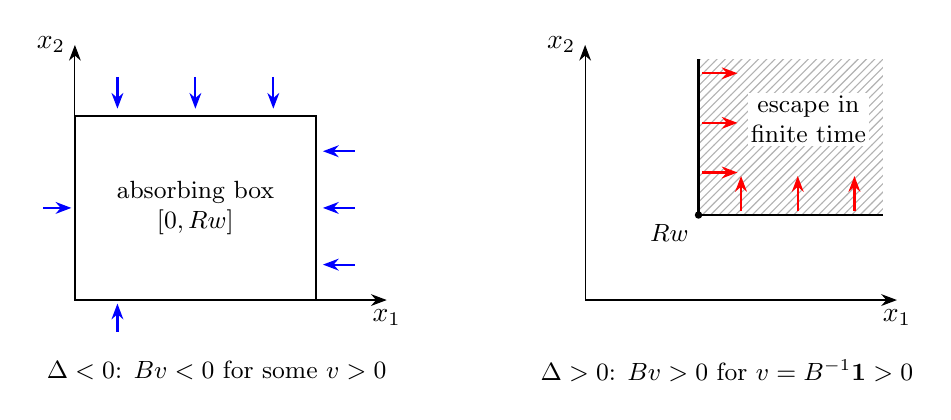
\begin{tikzpicture}[scale=0.9,>={Stealth[length=2mm]}]
 \begin{scope}
  \draw[->] (0,0) -- (4.4,0) node[below] {$x_1$};
  \draw[->] (0,0) -- (0,3.6) node[left] {$x_2$};
  \draw[thick] (0,0) rectangle (3.4,2.6);
  \foreach \y in {0.5,1.3,2.1} \draw[->,thick,blue] (3.95,\y) -- (3.5,\y);
  \foreach \x in {0.6,1.7,2.8} \draw[->,thick,blue] (\x,3.15) -- (\x,2.7);
  \draw[->,thick,blue] (0.6,-0.45) -- (0.6,-0.05);
  \draw[->,thick,blue] (-0.45,1.3) -- (-0.05,1.3);
  \node[align=center,font=\small] at (1.7,1.3) {absorbing box\\$[0,Rw]$};
  \node[font=\small] at (2.0,-1.0) {$\Delta<0$: $Bv<0$ for some $v>0$};
 \end{scope}
 \begin{scope}[xshift=7.2cm]
  \draw[->] (0,0) -- (4.4,0) node[below] {$x_1$};
  \draw[->] (0,0) -- (0,3.6) node[left] {$x_2$};
  \fill[pattern=north east lines,pattern color=gray!60] (1.6,1.2) rectangle (4.2,3.4);
  \draw[thick] (4.2,1.2) -- (1.6,1.2) -- (1.6,3.4);
  \foreach \x in {2.2,3.0,3.8} \draw[->,thick,red] (\x,1.25) -- (\x,1.75);
  \foreach \y in {1.8,2.5,3.2} \draw[->,thick,red] (1.65,\y) -- (2.15,\y);
  \fill (1.6,1.2) circle (1.5pt) node[below left,font=\small] {$Rw$};
  \node[align=center,font=\small,fill=white,inner sep=1pt] at (3.15,2.55) {escape in\\finite time};
  \node[font=\small] at (2.0,-1.0) {$\Delta>0$: $Bv>0$ for $v=B^{-1}\mathbf 1>0$};
 \end{scope}
\end{tikzpicture}
\caption{The dichotomy in a two-dimensional slice, with $w=1/v$. Left: the upper
faces of the box point inward and the lower faces, where $f_i\ge a_i>0$, point
inward too, so every positive solution enters the box. Right: on the lower faces
of the upper orthant beyond $Rw$ the field points outward, and solutions starting
there leave every bounded set in finite time.}
\label{fig:dichotomy}
\end{figure}

\section{Matrix alternatives and rectangular barriers}\label{sec:barriers}
We give the estimates explicitly because off-diagonal derivatives of $f$ need
not have a fixed sign. A global comparison theorem for cooperative vector
fields is therefore unnecessary.

\begin{lemma}[Matrix alternative]\label{lem:matrix}
For a matrix $B$ with positive diagonal and strictly negative off-diagonal entries:
if $\det B>0$, then $B^{-1}\one>0$; if $\det B<0$, there exists $v>0$ with $Bv<0$.
For weakly negative off-diagonal entries and nonnegative diagonal, $\det B>0$
still implies the first conclusion and a positive diagonal.
\end{lemma}
\begin{proof}
Write $B=D(I-A)$ with $D$ its positive diagonal and $A$ entrywise nonnegative
with zero diagonal. In the strict case $A$ is irreducible. Its characteristic
polynomial is $t^3-St-T$, where $S,T>0$, so it has exactly one positive real root,
its Perron root $\rho$. The remaining two eigenvalues are either both negative
or a conjugate pair; hence $\det(I-A)$ has the sign of $1-\rho$. If
$\det B>0$, then $\rho<1$ and $(I-A)^{-1}=\sum_{n\ge0}A^n\ge I$.
If $\det B<0$, a positive Perron vector satisfies
$Bv=(1-\rho)Dv<0$.

For the weak case expand the determinant, writing the off-diagonal magnitudes
as $m_{ij}\ge0$ and the diagonal as $q_i\ge0$:
\begin{align*}
\det B={}&q_1q_2q_3-q_1m_{23}m_{32}-q_2m_{13}m_{31}
-q_3m_{12}m_{21}\\
&-m_{12}m_{23}m_{31}-m_{13}m_{21}m_{32}.
\end{align*}
A positive determinant forces each $q_i>0$ and all principal two-by-two minors
positive. The diagonal cofactors are therefore positive and all off-diagonal
cofactors in the adjugate nonnegative. Thus $B^{-1}\one>0$.
\end{proof}

\begin{proposition}[An inward quadratic direction gives an absorbing box]\label{prop:inward}
For a strict system, if $Bv<0$ for some $v>0$, there is an absorbing box.
\end{proposition}
\begin{proof}
Set $w_i=1/v_i$, so $Q_i(w)<0$. For a fixed $i$ put
\[
 U_i=d_{ij}w_iw_j,\quad V_i=d_{ik}w_iw_k,\quad W_i=e_iw_jw_k,
 \quad \delta_i=\min\{U_i,V_i,(U_i+V_i-W_i)/2\}>0.
\]
The bilinear function
$-U_i u-V_i v+W_iuv+\delta_i(u+v)$ is nonpositive at all four corners of
$[0,1]^2$, and consequently throughout that square. On the upper face
$x_i=rw_i$, $x_j=rw_ju$, $x_k=rw_kv$, with $0\le u,v\le1$, it follows that
\[
 f_i(x)\le a_i-b_irw_i-\delta_i r^2(u+v)
              +r(c_{ij}w_ju+c_{ik}w_kv).
\]
Choose
\[
 R_1=\max_i\frac{\max(c_{ij}w_j,c_{ik}w_k)}{\delta_i},\quad
 A_0=\max_i a_i/w_i,\quad b_0=\min_i b_i>0.
\]
For $r(x)=\max_i x_i/w_i\ge R_1$, the upper Dini derivative obeys
\[
 D^+r\le A_0-b_0r.
\]
Thus every positive solution is bounded, cannot cease to exist in finite time,
and eventually enters any box $[0,Rw]$ with
$R>\max\{R_1,2A_0/b_0\}$. Such a box is positively invariant. The lower faces
point strictly inward because $a_i>0$ and all remaining terms in $f_i|_{x_i=0}$
are nonnegative. This also ensures forward invariance of the positive orthant.
\end{proof}

\begin{proposition}[An outward quadratic direction gives finite-time escape]\label{prop:outward}
In the weak sign class, if $Bv>0$ for some $v>0$, an open upper orthant of
initial points has finite maximal forward existence time.
\end{proposition}
\begin{proof}
Set $w_i=1/v_i$ and $\gamma=\min_i Q_i(w)/w_i>0$.
On a lower face $x_i=rw_i$, $x_j=rw_ju$, $x_k=rw_kv$ of the upper orthant,
$u,v\ge1$. With $U_i,V_i,W_i$ as above, $W_i>U_i+V_i$. Therefore
$-U_i u-V_i v+W_iuv$ is increasing in each variable on $[1,\infty)^2$,
and is bounded below by $Q_i(w)>0$. The affine terms give
\[
 \frac{f_i(x)}{w_i}\ge \frac{Q_i(w)}{w_i}r^2-b_ir.
\]
Consequently, for $r(x)=\min_i x_i/w_i$ and $b_* =\max_i b_i$,
its lower Dini derivative satisfies
$D_+r\ge\gamma r^2-b_*r$.
If $r(0)>2b_*/\gamma$, then $r$ increases and
$D_+r\ge\gamma r^2/2$. Integrating the reciprocal inequality shows that the
maximal forward existence time is at most $2/(\gamma r(0))$. A polynomial ODE
with a bounded solution extends past any finite time; hence finite maximal
existence time is finite-time escape in norm. No claim about an exact escape
profile or divergence of each individual coordinate is needed.
\end{proof}

\section{Degree and the sharp bound}\label{sec:degree}
The preceding barriers prove the dynamical assertions in the main theorem.
We now compute the degree. Only the positive-determinant case requires a
homotopy argument.

\begin{lemma}[Uniform compactness of positive zeros]\label{lem:compact}
For a compact family of strict systems with $\det B\ne0$ throughout, all
positive zeros lie in a common compact subset of the positive orthant.
\end{lemma}
\begin{proof}
Let every coefficient magnitude lie in $[\eta,M]$ with $\eta>0$.
At a positive zero,
\[
 x_i=\frac{a_i+c_{ij}x_j+c_{ik}x_k+e_ix_jx_k}
            {b_i+d_{ij}x_j+d_{ik}x_k}
 \le K\min\{1+x_j,1+x_k\},\qquad K=M/\eta.
\]
If one coordinate tends to infinity along a sequence of positive zeros, all
three tend to infinity and their ratios stay bounded above and below. Let
$H=\max_i x_i$. Then $H/x_i$ lies in a fixed compact subset of $(0,\infty)$.
Dividing $f=0$ by $x_1x_2x_3$ and multiplying by $H$ gives
\[
 B(H/x_1,H/x_2,H/x_3)^T=o(1).
\]
A subsequence yields a nonzero positive vector in the kernel of a limiting $B$,
contradicting nonsingularity. Hence positive zeros are uniformly bounded above.
They cannot approach a coordinate hyperplane, since on a bounded set the limit
of $f_i$ at $x_i=0$ is at least $\eta>0$.
\end{proof}

\begin{lemma}[Degree in the positive-determinant region]\label{lem:degree0}
Every strict system with $\det B>0$ has degree zero on a bounded open domain
containing all its positive zeros.
\end{lemma}
\begin{proof}
Positive multiplication of equations preserves their zeros and degree signs.
Normalise the diagonal of $B$ to one, obtaining $B=I-A$ with $A$ positive off
the diagonal and $\rho(A)<1$. Scale $A$ down through positive multiples until
its maximum row sum is less than $1/4$. Then interpolate it to the matrix
with all off-diagonal entries $1/10$; each intermediate row sum is less than one,
so $\rho<1$ throughout. Keep all lower-degree coefficients positive, and
interpolate them to reach the symmetric system
\[
 g_i=1-x_i+\tfrac1{10}(x_j+x_k)
            -\tfrac1{10}x_i(x_j+x_k)+x_jx_k.
\]
These paths stay inside the strict positive-determinant region. By
Lemma~\ref{lem:compact}, a common bounded degree domain exists along the entire
path, so the degree is constant. At a positive zero of $g$,
\[
 g_i-g_j=(x_j-x_i)\tfrac{11}{10}(1+x_k)=0,
\]
which forces all coordinates equal. But the diagonal equation is
$1-\tfrac45 t+\tfrac45 t^2=0$, whose discriminant is negative. The endpoint
has no positive zeros and therefore degree zero.
\end{proof}

\begin{proof}[Proof of Theorem~\ref{thm:main}]
If $\Delta<0$, Lemma~\ref{lem:matrix} and Proposition~\ref{prop:inward} give a
large invariant box with strictly inward upper faces. On its lower faces
$f_i>0$. The straight homotopy from $f$ to $h(x)=c-x$, with $c$ in the box's
interior, has no boundary zeros: on each face its normal component keeps the
same strict sign. Hence the degree is $\degB(h)=-1$.
By excision it can also be computed on a domain with closure in the positive
orthant. If $\Delta>0$, use Lemma~\ref{lem:degree0} for the degree and
Proposition~\ref{prop:outward}, with $v=B^{-1}\one$, for finite-time escape.

For regular systems the zero set is compact and discrete, hence finite, and
the degree equals the sum of Jacobian determinant signs. Reduction modulo two
therefore gives odd parity for $\Delta<0$ and even parity for $\Delta>0$.
The Newton polytope is
\[
 P=[0,1]^3\cap\{u_1+u_2+u_3\le2\}.
\]
It is a unit cube minus a tetrahedron of volume $1/6$, so $3!\operatorname{Vol}P=5$.
Bernstein's bound \cite{Bernstein}, or its perturbative upper-bound form for
nondegenerate roots, gives at most five isolated nondegenerate positive zeros.
Combining this bound with parity proves the stated lists.
\end{proof}

\begin{proof}[Proof of the sparse extension in Corollary~\ref{cor:sparse}]
The dynamical claim follows from Lemma~\ref{lem:matrix} and
Proposition~\ref{prop:outward}. For the root bound, suppose five
nondegenerate positive zeros existed. They persist under all sufficiently
small coefficient perturbations. Perturb into the strict class while preserving
$\det B>0$, and choose a generic perturbation so that all positive zeros are
nondegenerate. Such perturbations exist densely, since the singular systems
lie in the algebraic discriminant locus; independent constant perturbations
also give transversality directly. The strict system would then have at least
five positive zeros, contradicting the even bound four. Sharpness is proved
in the next section.
\end{proof}

\section{A seven-reaction witness and an explicit escape region}\label{sec:seven}
Consider the reactions
\begin{center}
\begin{tabular}{lr@{\qquad}lr}
\toprule
Reaction & Rate & Reaction & Rate\\\midrule
$X_1+X_2\to0$ & 7 & $X_2+X_3\to X_1+X_2+X_3$ & 1\\
$X_1+X_3\to X_2+X_3$ & 1 & $0\to X_2$ & 1\\
$X_3\to X_1$ & 1 & $X_1\to X_1+X_3$ & 3\\
$X_1+X_2\to X_3$ & 1 & &\\\bottomrule
\end{tabular}
\end{center}
Quadratic refers to reactant degree, as in \cite{TZ}; a product may contain
three species. The stoichiometric rank is three, as witnessed by the vectors
$(0,1,0),(1,0,-1),(0,0,1)$.

Writing concentrations as $(x,y,z)$ gives
\begin{equation}\label{eq:seven}
 f=(-8xy-xz+z+yz,\ -8xy+xz+1,\ xy-z+3x).
\end{equation}
The identity $f_2+8f_3=x(z+24)-(8z-1)$ shows that any positive zero has
\[
 z>1/8,\qquad x=\frac{8z-1}{z+24},\qquad
 y=\frac{z^2+3}{8z-1}.
\]
The last two equations then vanish identically, and the first is
\[
 f_1=\frac{P(z)}{(z+24)(8z-1)},\qquad
 P(z)=z^4-96z^3+218z^2-145z+24.
\]
Exactly,
\[
 \big(P(1/8),P(1/2),P(1),P(2),P(96)\big)
 =\big(37249/4096,-95/16,2,-146,1995192\big).
\]
Four disjoint sign changes (Figure~\ref{fig:signs}) prove that all four roots
are simple and larger than $1/8$. They give exactly four positive steady states.
The minor $\det\partial(f_2,f_3)/\partial(x,y)=x(z+24)>0$ yields, by
differentiation along the eliminated curve,
\[
 \det Df=\frac{P'(z)}{z+24}\quad\hbox{at every steady state}.
\]
This proves nondegeneracy and signs $-,+,-,+$ independently of determinant
alternation. Direct rational Routh--Hurwitz certificates verify two stable
states. For the characteristic coefficients $b_1,b_2,b_3$ and
$H_2=b_1b_2-b_3$, the first state has enclosures
$(26,27),(6,7),(2,3),(179,180)$ and the third has
$(9,10),(13,14),(1,2),(125,126)$, respectively.

The behaviour at infinity is equally explicit:
\[
 B=\begin{pmatrix}1&-1&-8\\0&1&-8\\0&0&1\end{pmatrix},\quad
 B^{-1}\one=(18,9,1)^T,\quad w=(1/18,1/9,1)^T.
\]
Here $Q_i(w)=1/162$, $\gamma=1/162$, and $b_*=1$. The proof of
Proposition~\ref{prop:outward} gives
\begin{equation}\label{eq:escape}
 r_0=\min\{18x(0),9y(0),z(0)\}>324
 \quad\Longrightarrow\quad T_{\max}\le324/r_0<1.
\end{equation}
Thus two attracting equilibria coexist with an open region of finite-time
escape. Local multistability alone does not imply global boundedness.

Using \cite[Theorem 2]{TZ}, the least number of reactions for four nondegenerate
positive steady states is seven. The theorem excludes six. It is proved by real
root classification, which certifies counts for rate vectors off a discriminant
hypersurface, but it bounds every rate vector: four nondegenerate states at one
rate vector would persist on an open set of rate vectors, and an open set meets
the complement of a hypersurface. If a smaller network
had four such states, add unused quadratic zero-one reactions at sufficiently
small positive rates until there are six; nondegenerate positive states persist,
giving a contradiction. This lower-bound argument relies on the cited
computer-assisted theorem; the witness and escape proof do not.

\section{Five steady states with eight reactions}\label{sec:five}
Consider the reactions
\begin{center}
\begin{tabular}{lr@{\qquad}lr}
\toprule
Reaction & Rate & Reaction & Rate\\\midrule
$X_1\to X_1+X_3$ & 5 & $X_2+X_3\to X_1$ & $2/5$\\
$X_1\to X_2$ & 1 & $X_3\to0$ & $1/2$\\
$X_1+X_3\to X_1+X_2+X_3$ & 1 & $0\to X_1+X_2$ & $1/2500$\\
$X_1+X_2\to X_2$ & 1 & $X_2\to X_1$ & $1/100000$\\\bottomrule
\end{tabular}
\end{center}
The network is quadratic zero-one with stoichiometric rank three. With
concentrations $(x,y,z)$ the mass-action system is
\begin{equation}\label{eq:eight}
\begin{aligned}
 f_1&=\tfrac1{2500}-x-xy+\tfrac25yz+\tfrac1{100000}y,\\
 f_2&=\tfrac1{2500}+x+xz-\tfrac25yz-\tfrac1{100000}y,\\
 f_3&=5x-\tfrac12z-\tfrac25yz.
\end{aligned}
\end{equation}

\begin{theorem}\label{thm:five}
The system \eqref{eq:eight} has exactly five positive steady states. All five
are nondegenerate, with $\det Df$ of signs $-,+,-,+,-$ in increasing $z$; three
are asymptotically stable and two are unstable.
\end{theorem}

\begin{proof}
The equation $f_3=0$ is linear in $x$ and gives $50x=z(5+4y)$. Substituting this
into $f_2$ leaves an expression linear in $y$:
\[
 100000\,f_2=y\,D(z)+N(z),\qquad D(z)=8000z^2-32000z-1,\quad N(z)=10000z^2+10000z+40.
\]
At a positive steady state $N(z)>0$, so $D(z)\ne0$ and
\[
 y=Y(z)=-\frac{N(z)}{D(z)},\qquad x=X(z)=\frac{z\,(5+4Y(z))}{50}.
\]
Conversely, these two formulas make $f_2$ and $f_3$ vanish identically wherever
$D(z)\ne0$, so the curve $f_2=f_3=0$ is rational with parameter $z$. Substituting
into the remaining equation gives
\[
 f_1(X(z),Y(z),z)=-\frac{E(z)}{1250\,D(z)^2},
\]
\[
 E(z)=40000000000z^5-110031000000z^4+50416250000z^3-782738125z^2+101000z-1.
\]
Positive steady states therefore correspond to the roots $z>0$ of $E$ at which
$X$ and $Y$ are positive. The exact values
\[
\begin{array}{c|cccccc}
 z & 0 & \tfrac1{20000} & \tfrac1{1000} & \tfrac1{10} & 1 & 3\\\hline
 E(z) & -1 & \tfrac{335912964971}{160000000000} & -\tfrac{316215933}{500000}
      & \tfrac{127983471}{4} & -20397387126 & 2161683409874
\end{array}
\]
alternate in sign (Figure~\ref{fig:signs}), so $E$ has a root in each of the five intervals they bound.
A quintic has no others, and each of these roots is simple. All five lie in
$(0,3)$, where $D<0$; hence $Y>0$ and $X>0$ there. This proves the count.

For the determinant, the two-by-two minor of $Df$ in the variables $(x,y)$ for
the equations $(f_2,f_3)$ is
\[
 M(z)=\det\frac{\partial(f_2,f_3)}{\partial(x,y)}
     =\tfrac85z-\tfrac25z^2+\tfrac1{20000},
\]
which is positive on $(0,4)$. Differentiating along the curve, as in
Section~\ref{sec:seven}, gives at every root of $E$
\[
 \det Df=-\frac{M(z)\,E'(z)}{1250\,D(z)^2}.
\]
At the five simple roots $E'$ has the signs $+,-,+,-,+$ of the crossings, which
gives the stated determinant signs. Stability of the first, third and fifth
states is certified by exact rational Routh--Hurwitz enclosures, computed by the
same verifier as in Section~\ref{sec:seven}; states with $\det Df>0$ have a positive real
eigenvalue.
\end{proof}

\begin{figure}[ht]
\centering
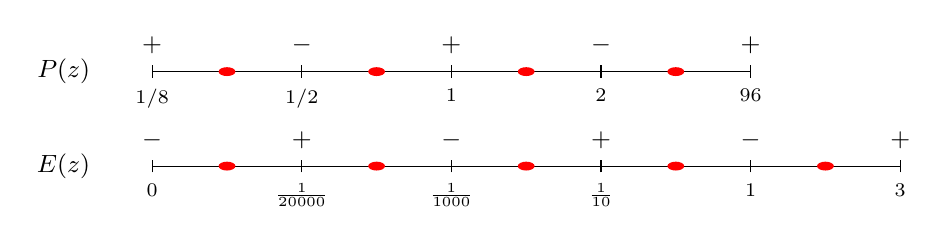
\begin{tikzpicture}[xscale=1.9,yscale=1]
 \node[anchor=east,font=\small] at (-0.35,1.2) {$P(z)$};
 \draw (0,1.2) -- (4,1.2);
 \foreach \x/\l/\s in {0/{1/8}/+,1/{1/2}/-,2/1/+,3/2/-,4/96/+} {
   \draw (\x,1.12) -- (\x,1.28); \node[below,font=\scriptsize] at (\x,1.1) {$\l$};
   \node[above,font=\small] at (\x,1.3) {$\s$};}
 \foreach \x in {0.5,1.5,2.5,3.5} \fill[red] (\x,1.2) circle (1.6pt);
 \node[anchor=east,font=\small] at (-0.35,0) {$E(z)$};
 \draw (0,0) -- (5,0);
 \foreach \x/\l/\s in {0/0/-,1/{\frac1{20000}}/+,2/{\frac1{1000}}/-,3/{\frac1{10}}/+,4/1/-,5/3/+} {
   \draw (\x,-0.08) -- (\x,0.08); \node[below,font=\scriptsize] at (\x,-0.1) {$\l$};
   \node[above,font=\small] at (\x,0.1) {$\s$};}
 \foreach \x in {0.5,1.5,2.5,3.5,4.5} \fill[red] (\x,0) circle (1.6pt);
\end{tikzpicture}
\caption{Sign diagrams, not to scale. Top: the quartic $P$ of Section~\ref{sec:seven}
changes sign four times on $(1/8,\infty)$, giving the four steady states of the
seven-reaction network. Bottom: the quintic $E$ of Section~\ref{sec:five} changes sign
five times on $(0,3)$, giving the five steady states of the eight-reaction network.
Dots mark the roots.}
\label{fig:signs}
\end{figure}

The coordinates are approximately $(2.68\times10^{-5},\,29.80,\,1.08\times10^{-5})$,
$(9.35\times10^{-5},\,8.554,\,1.19\times10^{-4})$, $(0.00210,\,0.3966,\,0.01595)$,
$(0.0814,\,0.5690,\,0.5591)$ and $(0.5964,\,2.177,\,2.176)$. These values play no
part in the proof.

The quadratic coefficient matrix is
\[
 B=\begin{pmatrix}2/5&0&-1\\-2/5&1&0\\-2/5&0&0\end{pmatrix},\qquad \det B=-\tfrac25<0.
\]
The system is sparse, so Theorem~\ref{thm:main} does not apply to it directly.
Its five nondegenerate states persist under every sufficiently small strict
perturbation, which keeps $\det B<0$, so those strict systems are regular
five-state systems in the absorbing-box region, as Corollary~\ref{cor:fourfive}
requires. The construction also explains where the example came from. The
seven-reaction network obtained by deleting $X_2\to X_1$ has four positive steady
states and a negative quadratic determinant. Corollary~\ref{cor:reduction} and
the parity statement then force a fifth state in any small strict perturbation,
and adding the single reaction $X_2\to X_1$ at a small rate is enough to produce it.

\section{Strict sharpness and exact reproducibility}
In monomial order $(1,x,y,z,xy,xz,yz)$, a strict integer coefficient matrix
attaining four positive steady states is
\begin{equation}\label{eq:strictfour}
 C=\begin{pmatrix}
 1&-1&1&101&-801&-101&101\\
 101&1&-1&1&-801&101&-1\\
 1&301&1&-101&101&-1&-1
 \end{pmatrix}.
\end{equation}
It is obtained by multiplying \eqref{eq:seven} by 100 and adding one unit in
every prescribed coefficient direction. Its quadratic determinant is $776596>0$.
Exact lexicographic elimination gives a squarefree quintic; all five roots are
real, one negative and four positive. The latter lift to positive coordinates,
with determinant signs $-,+,-,+$. Rational root isolation and interval sign
checks certify the count and two stable states. This proves sharpness inside
the strict class, rather than just on its boundary.

The accompanying verifier checks strict examples with $N=0,1,2,3,4$,
including the predicted determinant signs, degree sums, and exact inward or
outward barrier inequalities. The three-state strict witness is a perturbation
of \cite[Example 3]{TZ}, not a separate new topology. Full coefficient matrices,
exact root certificates and verification commands are at~\cite{repo}.

\section{Formal verification}
Both extreme examples are verified in Lean~4 with Mathlib \cite{Lean4,Mathlib}.
For each network the formal statement derives the mass-action system from the
reaction list, proves that the stated Jacobian entries are the partial
derivatives, and proves that the set of positive steady states consists of
exactly four, respectively five, explicit points, each in a stated rational
interval, with determinant signs $-,+,-,+$ and $-,+,-,+,-$. The proofs follow
Sections~\ref{sec:seven} and~\ref{sec:five}: the rational curve, the sign changes of the
eliminant, the bound on the number of roots of a polynomial, and the determinant
identity. They use only the standard axioms of Lean's logic. Each formalisation
was tested against planted errors (a wrong count, a wrong sign, a changed rate, a
wrong Jacobian entry, a shifted root interval); all of the 10 and 11 planted
variants respectively fail to compile. The stability counts, which rely on the
Routh--Hurwitz criterion, are certified by exact rational arithmetic but are not
formalised. The general dichotomy is not formalised; its degree-theoretic steps
use the standard properties of the Brouwer degree.

\section{What remains open}\label{sec:open}
The least number of reactions admitting five positive steady states is seven or
eight. Eight is attained by Theorem~\ref{thm:five}. Seven is not excluded: the
mixed volume of the steady-state supports already reaches five for some
seven-reaction networks. The construction of Section~\ref{sec:five} starts from a
seven-reaction network with four states and so cannot produce a seven-reaction
example; we have not found one by other means.

The hypersurface $\Delta=0$ and systems with vanishing coefficient slots require
separate analysis for global dynamics and degree; the sparse upper bound and the
finite-time-escape criterion are the stated exceptions. The four-state network
obtained by deleting $X_2\to X_1$ from Section~\ref{sec:five} has $\det B<0$ and an
even count, so the parity statement genuinely needs the strict class.
Extending the matrix $B$ and the dichotomy beyond three species is a natural
next step that this paper does not attempt.

Two other literatures meet these arguments. The barriers of Section~3 check
bilinear functions at the corners of box faces. This is the vertex principle for
multi-affine vector fields on rectangles, used for control by Belta and Habets
\cite{BH} and extended to polynomial fields by Ben Sassi and Girard \cite{BSG};
here it is applied on boxes that grow without bound, where only the quadratic
part decides. Boundedness of mass-action systems can also follow from network
structure alone: strongly endotactic networks are permanent \cite{GMS}. That
criterion does not involve the rate constants. The determinant $\Delta$ does. In the
strict realisation each coefficient slot comes from its own reaction, so scaling
the rates of the reactions on the diagonal of $B$ moves $\Delta$ through zero in a
single network, and for such a network no rate-independent criterion can decide
boundedness. Classical dissipativity criteria for Lotka--Volterra systems
\cite{Takeuchi} concern quadratic parts of the form $x_i(Ax)_i$, which differ from
the reciprocal form \eqref{eq:reciprocal}.

Odd parity for dissipative networks without boundary equilibria is already part
of the general degree framework of Conradi et al.\ \cite{CFMW}; odd parity alone
is not a new claim here.
The proof uses standard Perron--Frobenius and Brouwer degree principles, together
with Bernstein's root bound; its proposed contribution is their explicit
coefficient-level combination for this sign class, the sharp bound in one
region, its connection with finite-time escape, and the two extreme examples.

\section*{Acknowledgements}
The question of why three steady states is the limit is Tang and Zhang's~\cite{TZ}.
Two AI systems were used in this work under the author's direction. OpenAI Codex
found the integer seven-reaction network of Section~\ref{sec:seven}, proposed the
determinant dichotomy and its proof, wrote the exact verifier and its certificates,
and drafted the first version of the text. Claude Opus~5.5 (Anthropic) audited that
draft and its proofs, found the eight-reaction five-state network and the elementary
proofs of both extreme examples, wrote the Lean formalisation and the independent
recheck, and revised the text. The author is responsible for the content of this
preprint, which has not yet been independently reviewed.

\begin{thebibliography}{9}
\bibitem{repo} V. Jandhyala, A determinant dichotomy for quadratic zero-one systems: code,
certificates and Lean proofs,
\url{https://github.com/jvvk/mathematics/tree/main/steady-state-dichotomy}.
\bibitem{TZ} X. Tang and J. Zhang,
\emph{The Ubiquity of Three Steady States: Minimal Multistable Zero-One Reaction Networks},
arXiv:2608.01116v1 (2026). \url{https://arxiv.org/abs/2608.01116}
(accessed 16 October 2026).
\bibitem{JTZ} Y. Jiao, X. Tang and X. Zeng,
\emph{Multistability of small zero-one reaction networks}, Journal of Mathematical
Biology \textbf{91}(6) (2025), article 82.
\url{https://doi.org/10.1007/s00285-025-02306-w}; preprint arXiv:2406.11586v2
(accessed 16 October 2026).
\bibitem{TW} X. Tang and K. Wang, \emph{Hopf bifurcations of reaction networks with
zero-one stoichiometric coefficients}, SIAM Journal on Applied Dynamical Systems
\textbf{22}(3) (2023), 2459--2489. \url{https://doi.org/10.1137/22M1519754}.
\bibitem{CFMW} C. Conradi, E. Feliu, M. Mincheva and C. Wiuf,
\emph{Identifying parameter regions for multistationarity}, PLoS Computational
Biology \textbf{13}(10) (2017), e1005751.
\url{https://doi.org/10.1371/journal.pcbi.1005751}.
\bibitem{Bernstein} D. N. Bernshtein,
\emph{The number of roots of a system of equations}, Functional Analysis and
Its Applications \textbf{9} (1975), 183--185.
\url{https://doi.org/10.1007/BF01075595}.
\bibitem{Lean4} L. de Moura and S. Ullrich,
\emph{The Lean 4 theorem prover and programming language}, in Automated
Deduction, CADE 28, Lecture Notes in Computer Science \textbf{12699} (2021),
625--635. \url{https://doi.org/10.1007/978-3-030-79876-5_37}.
\bibitem{Mathlib} The mathlib Community,
\emph{The Lean mathematical library}, in Proceedings of the 9th ACM SIGPLAN
International Conference on Certified Programs and Proofs (CPP 2020), 367--381.
\url{https://doi.org/10.1145/3372885.3373824}.
\bibitem{BH} C. Belta and L. C. G. J. M. Habets,
\emph{Controlling a class of nonlinear systems on rectangles}, IEEE Transactions
on Automatic Control \textbf{51}(11) (2006), 1749--1759.
\url{https://doi.org/10.1109/TAC.2006.884957}.
\bibitem{BSG} M. A. Ben Sassi and A. Girard,
\emph{Control of polynomial dynamical systems on rectangles}, in 2013 European
Control Conference (ECC), 658--663. \url{https://doi.org/10.23919/ECC.2013.6669360}.
\bibitem{GMS} M. Gopalkrishnan, E. Miller and A. Shiu,
\emph{A geometric approach to the global attractor conjecture}, SIAM Journal on
Applied Dynamical Systems \textbf{13}(2) (2014), 758--797.
\url{https://doi.org/10.1137/130928170}.
\bibitem{Takeuchi} Y. Takeuchi, \emph{Global Dynamical Properties of
Lotka--Volterra Systems}, World Scientific, Singapore, 1996.
\url{https://doi.org/10.1142/9789812830548}.
\end{thebibliography}
\end{document}
